El aprendizaje supervisado y no supervisado son dos enfoques fundamentales en el campo del aprendizaje automático, cada uno con sus propias características, aplicaciones y desafíos. El aprendizaje supervisado se basa en la utilización de datos etiquetados para entrenar modelos que puedan hacer predicciones o clasificaciones precisas. En contraste, el aprendizaje no supervisado se enfoca en descubrir patrones y estructuras ocultas en datos no etiquetados, lo que lo hace especialmente útil para tareas como la agrupación y la reducción de dimensionalidad. 
\begin{figure}[H]
    \begin{center}
    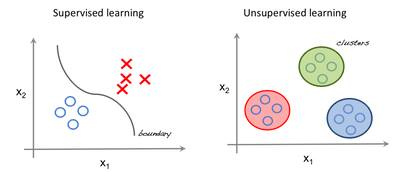
\includegraphics[width=0.7\textwidth]{commons/Fig5.jpg}
    \caption{Comparativa de clasificación entre aprendizaje supervisado y no supervisado. Imagen de Juan Domingo Farnos}
    \label{fig:SupervNoSuperv}
    \cite{rafii18}
    \end{center}
\end{figure}